% Sección de resultados: figuras construidas a partir de los nombres
% de archivo en la carpeta Imagenes/.
\section{Resultados}

%---------------------------------------------------------------
\subsection{Visualización en el dominio del tiempo y de la frecuencia de una onda sinusoidal}

\begin{figure}[H]
    \centering
    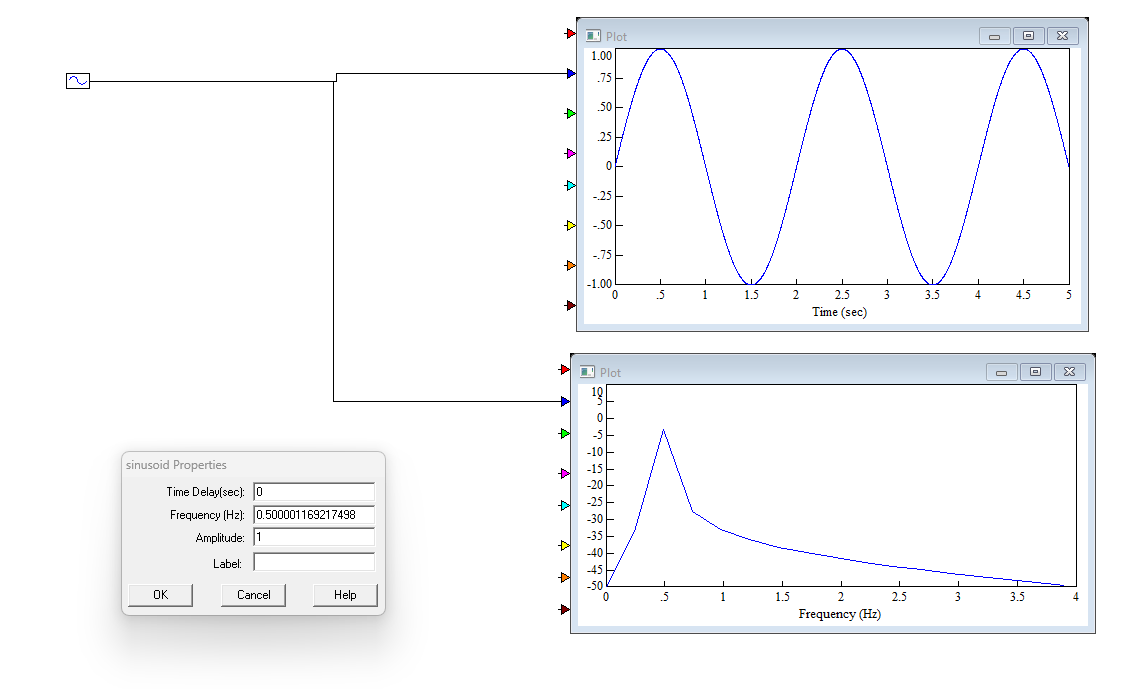
\includegraphics[width=0.6\textwidth]{Imagenes/parte-1-entrada-sinusoidal.png}
    \caption{Entrada sinusoidal en el dominio del tiempo}
    \label{fig:parte1-entrada-sinusoidal}
\end{figure}

%---------------------------------------------------------------
\subsection{Construcción de una señal modulada en amplitud con doble banda lateral y portadora}

\begin{figure}[H]
    \centering
    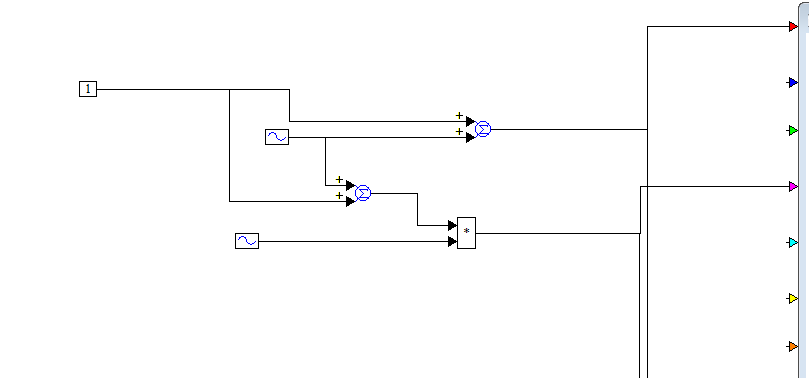
\includegraphics[width=0.6\textwidth]{Imagenes/parte-2-sistema-modulacion-AM.png}
    \caption{Sistema de modulación AM de doble banda lateral con portadora}
    \label{fig:parte2-sistema-modulacion-am}
\end{figure}

\begin{figure}[H]
    \centering
    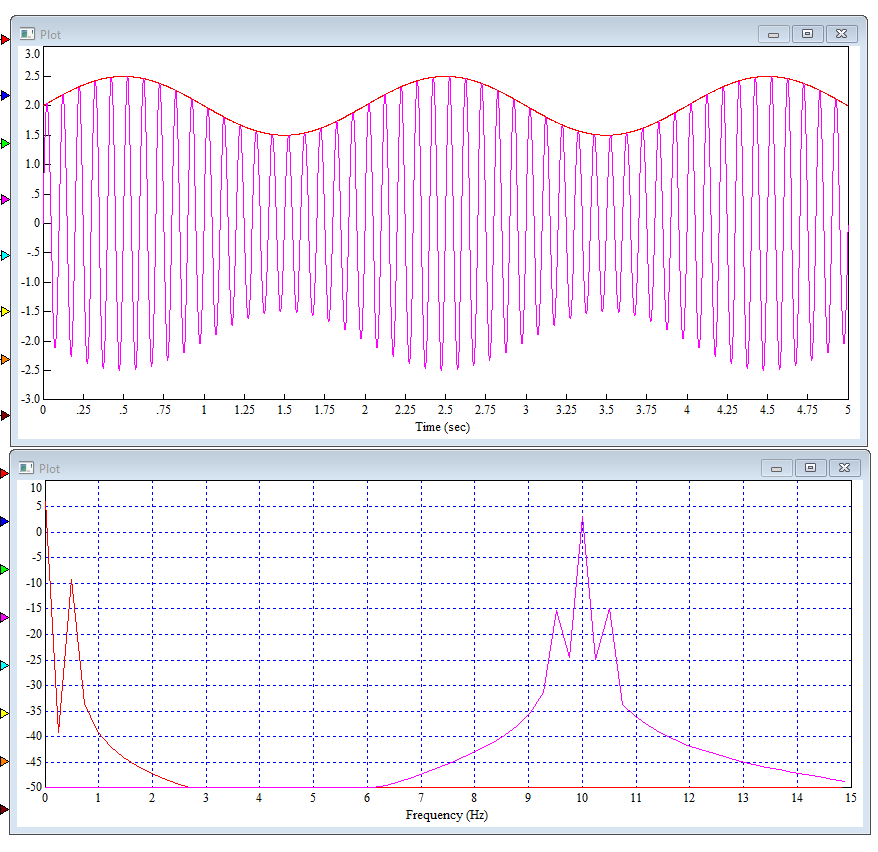
\includegraphics[width=0.6\textwidth]{Imagenes/parte-2-modulacion-indice-de-modulacion-0.25.png}
    \caption{Señal AM con índice de modulación 0{,}25}
    \label{fig:parte2-indice-modulacion-0-25}
\end{figure}

\begin{figure}[H]
    \centering
    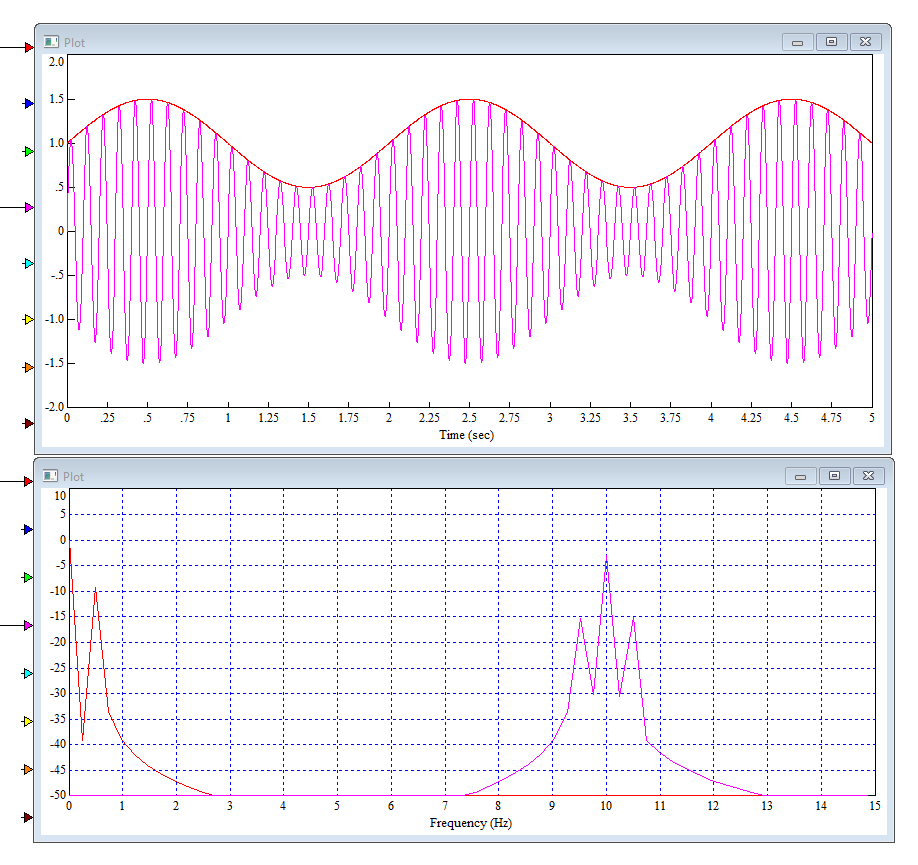
\includegraphics[width=0.6\textwidth]{Imagenes/parte-2-modulacion-indice-de-modulacion-0.5.png}
    \caption{Señal AM con índice de modulación 0{,}5}
    \label{fig:parte2-indice-modulacion-0-5}
\end{figure}

\begin{figure}[H]
    \centering
    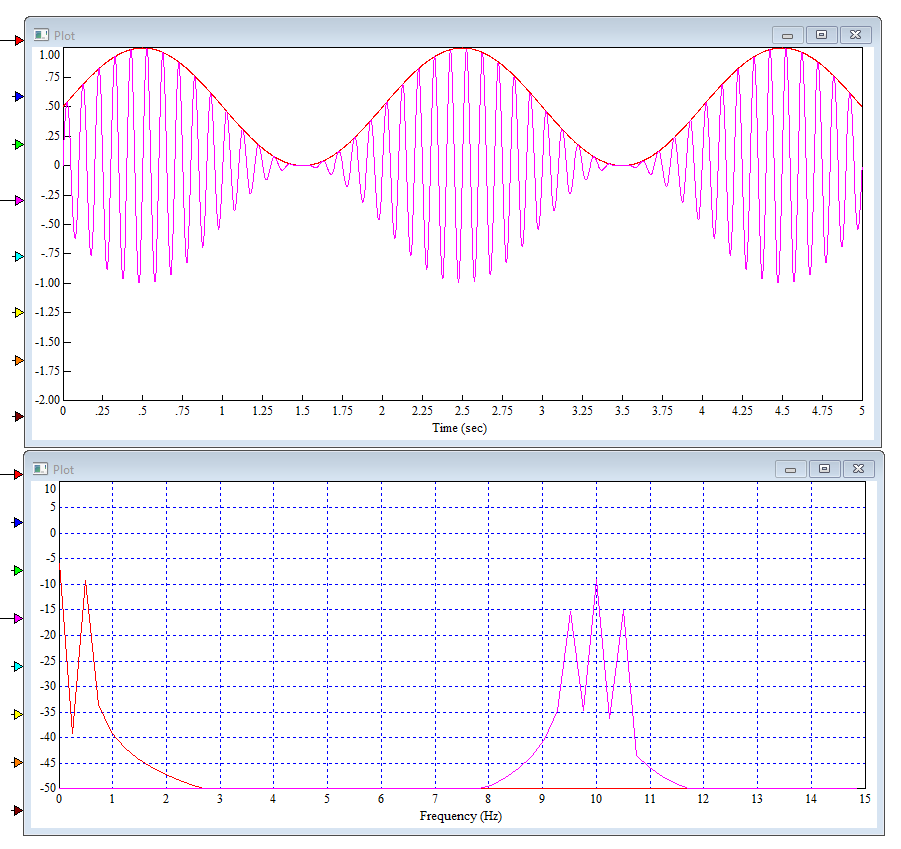
\includegraphics[width=0.6\textwidth]{Imagenes/Parte-2-indice-de-modulacion-1.png}
    \caption{Señal AM con índice de modulación 1}
    \label{fig:parte2-indice-modulacion-1}
\end{figure}

\begin{figure}[H]
    \centering
    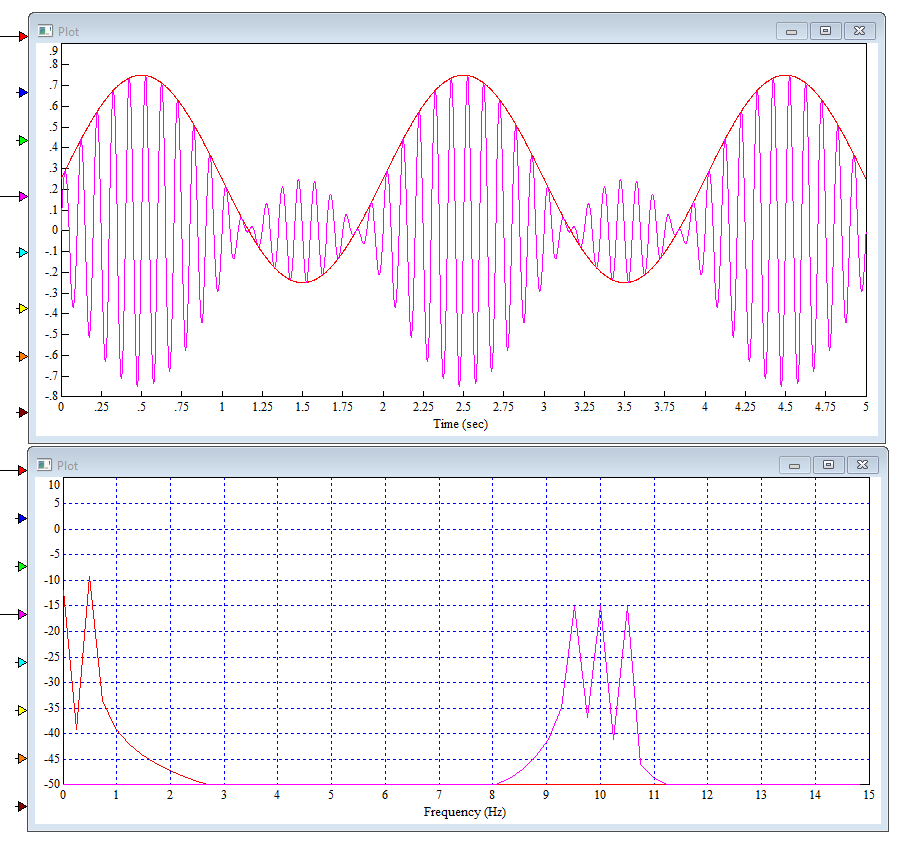
\includegraphics[width=0.6\textwidth]{Imagenes/Parte-2-modulacion-sobremodulacion.png}
    \caption{Señal AM en sobremodulación}
    \label{fig:parte2-sobremodulacion}
\end{figure}

%---------------------------------------------------------------
\subsection{Construcción de la señal modulada en amplitud con el generador de forma de onda}

% Sistema de modulación con generador de señales
\begin{figure}[H]
    \centering
    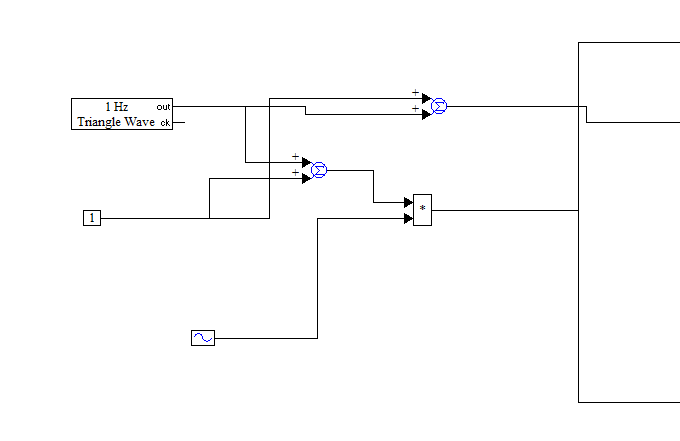
\includegraphics[width=0.6\textwidth]{Imagenes/parte-3-sistema-modulacion-am-generador-de-señales.png}
    \caption{Sistema de modulación AM implementado con el generador de señales}
    \label{fig:parte3-sistema-modulacion-am-generador}
\end{figure}

% Moduladora cuadrada
\begin{figure}[H]
    \centering
    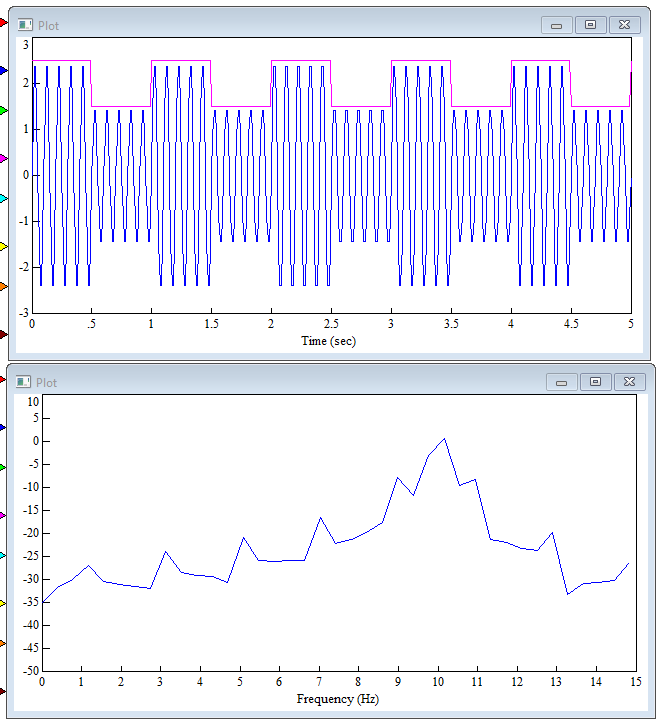
\includegraphics[width=0.6\textwidth]{Imagenes/Parte-3-moduladora-cuadrada-indice-de-modulacion-0.25.png}
    \caption{Señal AM con moduladora cuadrada e índice de modulación 0{,}25}
    \label{fig:parte3-cuadrada-indice-0-25}
\end{figure}

\begin{figure}[H]
    \centering
    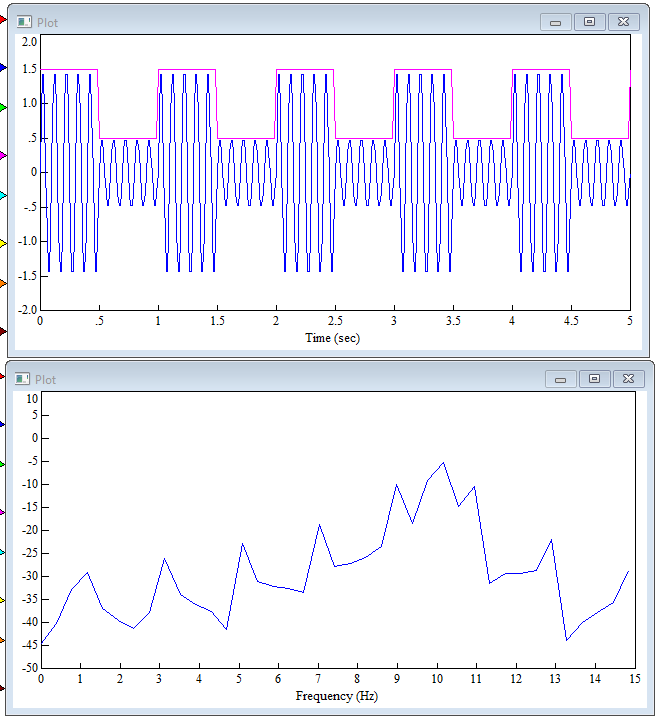
\includegraphics[width=0.6\textwidth]{Imagenes/Parte-3-moduladora-cuadrada-indice-de-modulacion-0.5.png}
    \caption{Señal AM con moduladora cuadrada e índice de modulación 0{,}5}
    \label{fig:parte3-cuadrada-indice-0-5}
\end{figure}

\begin{figure}[H]
    \centering
    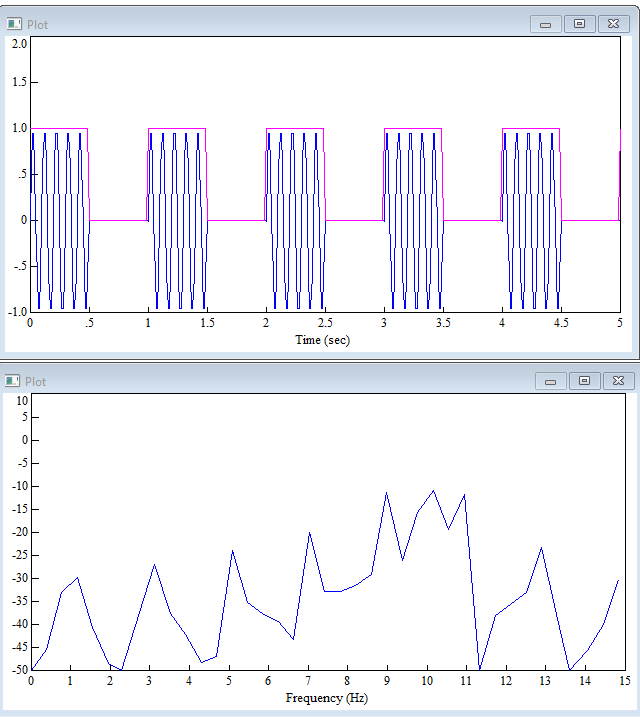
\includegraphics[width=0.6\textwidth]{Imagenes/Parte-3-moduladora-cuadrada-indice-de-modulacion-1.png}
    \caption{Señal AM con moduladora cuadrada e índice de modulación 1}
    \label{fig:parte3-cuadrada-indice-1}
\end{figure}

\begin{figure}[H]
    \centering
    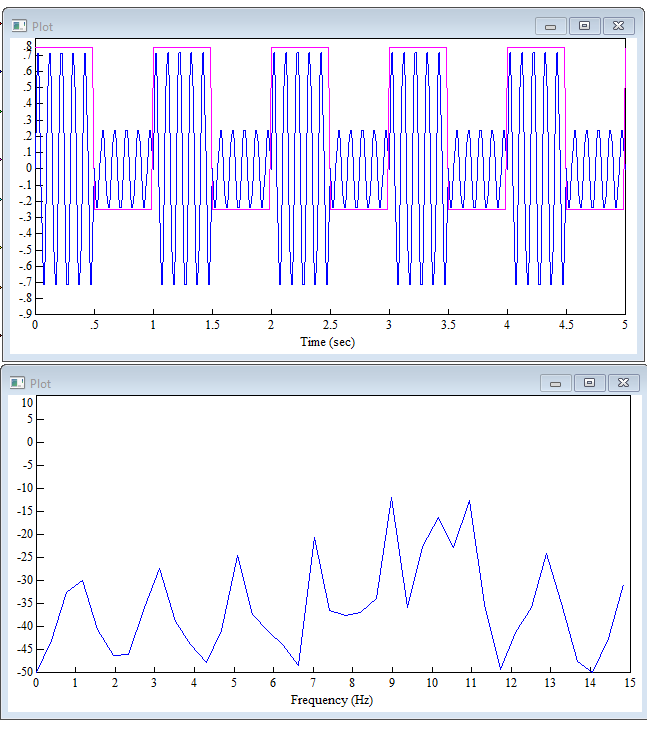
\includegraphics[width=0.6\textwidth]{Imagenes/Parte-3-moduladora-cuadrada-sobremodulacion.png}
    \caption{Señal AM con moduladora cuadrada en sobremodulación}
    \label{fig:parte3-cuadrada-sobremodulacion}
\end{figure}

% Moduladora diente de sierra
\begin{figure}[H]
    \centering
    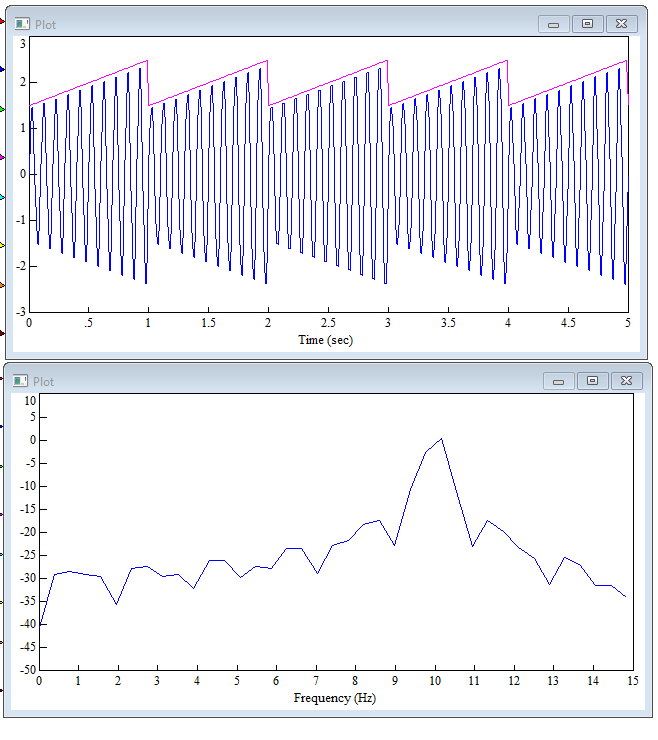
\includegraphics[width=0.6\textwidth]{Imagenes/Parte-3-moduladora-dientedecierra-indice-de-modulacion-0.25.png}
    \caption{Señal AM con moduladora diente de sierra e índice de modulación 0{,}25}
    \label{fig:parte3-diente-de-sierra-indice-0-25}
\end{figure}

\begin{figure}[H]
    \centering
    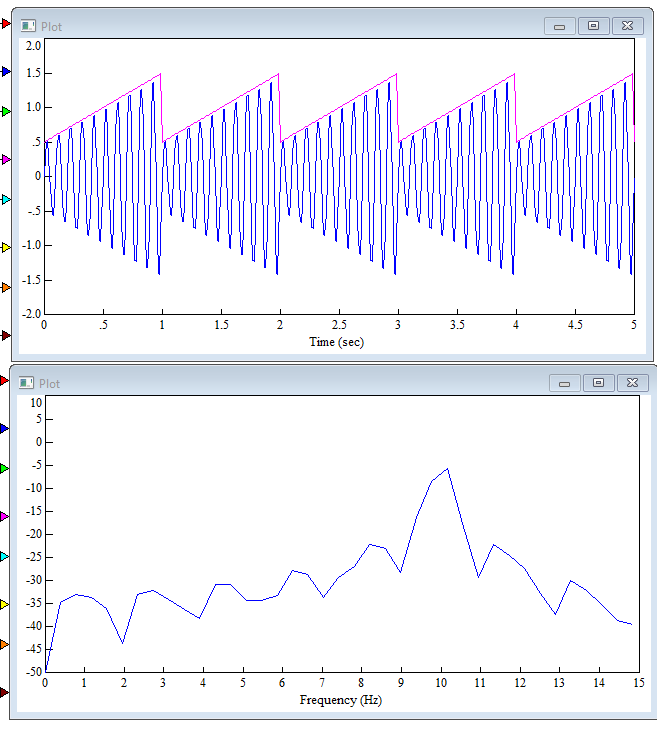
\includegraphics[width=0.6\textwidth]{Imagenes/Parte-3-moduladora-dientedecierra-indice-de-modulacion-0.5.png}
    \caption{Señal AM con moduladora diente de sierra e índice de modulación 0{,}5}
    \label{fig:parte3-diente-de-sierra-indice-0-5}
\end{figure}

\begin{figure}[H]
    \centering
    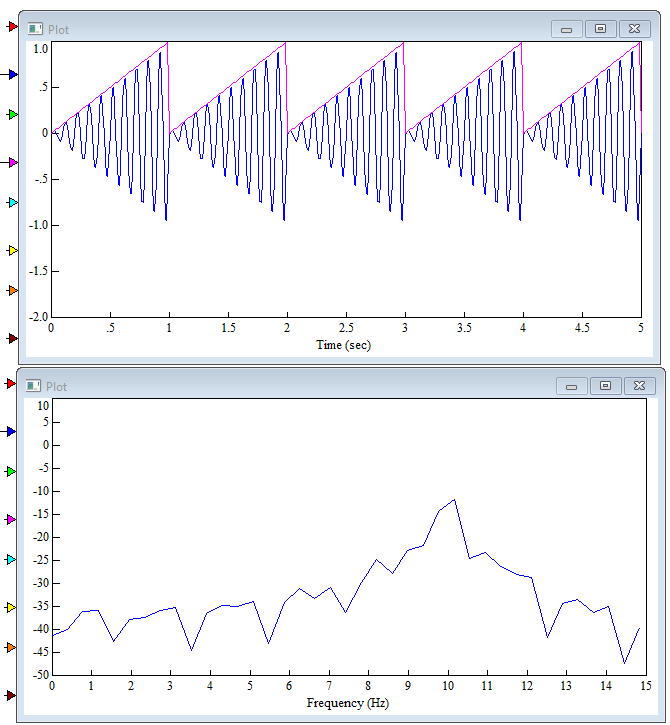
\includegraphics[width=0.6\textwidth]{Imagenes/Parte-3-moduladora-dientedesierra-indice-de-modulacion-1.png}
    \caption{Señal AM con moduladora diente de sierra e índice de modulación 1}
    \label{fig:parte3-diente-de-sierra-indice-1}
\end{figure}

\begin{figure}[H]
    \centering
    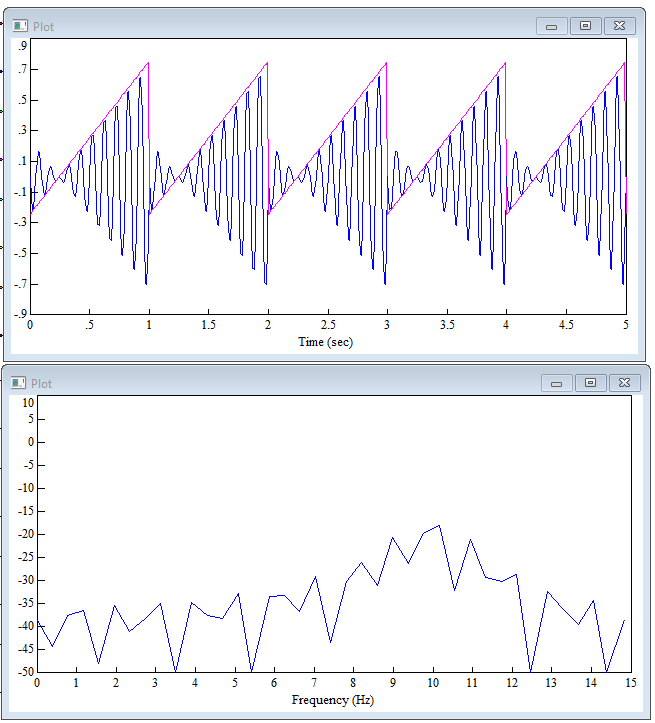
\includegraphics[width=0.6\textwidth]{Imagenes/Parte-3-moduladora-dientedesierra-sobremodulacion.png}
    \caption{Señal AM con moduladora diente de sierra en sobremodulación}
    \label{fig:parte3-diente-de-sierra-sobremodulacion}
\end{figure}

% Moduladora triangular
\begin{figure}[H]
    \centering
    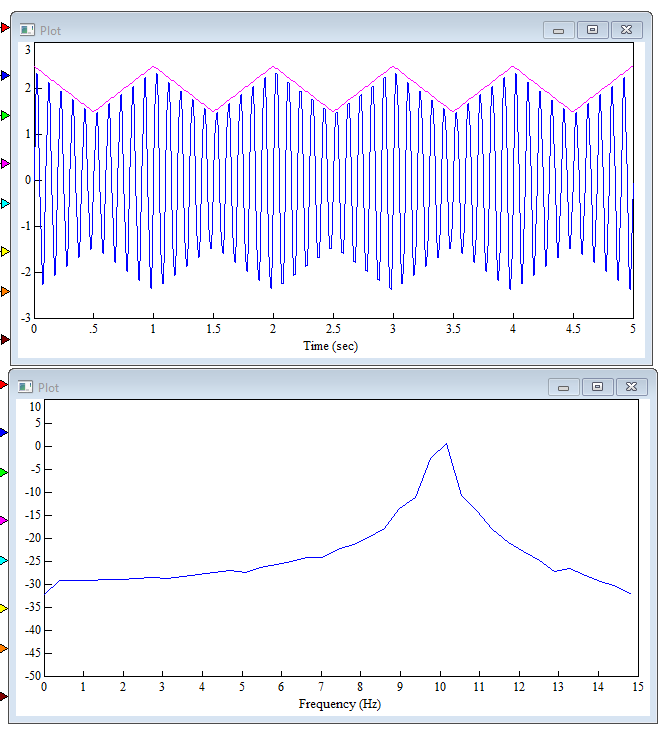
\includegraphics[width=0.6\textwidth]{Imagenes/Parte-3-moduladora-triangular-indice-de-modulacion-0.25.png}
    \caption{Señal AM con moduladora triangular e índice de modulación 0{,}25}
    \label{fig:parte3-triangular-indice-0-25}
\end{figure}

\begin{figure}[H]
    \centering
    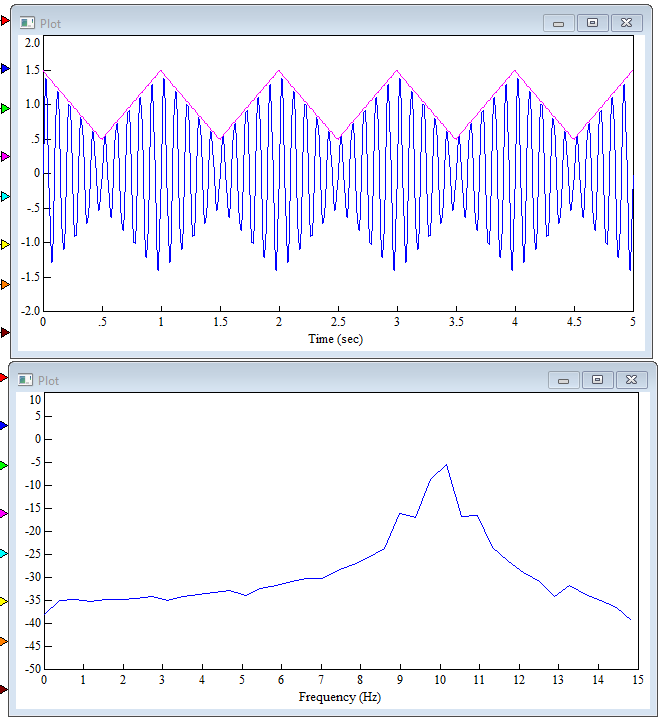
\includegraphics[width=0.6\textwidth]{Imagenes/Parte-3-moduladora-triangular-indice-de-modulacion-0.5.png}
    \caption{Señal AM con moduladora triangular e índice de modulación 0{,}5}
    \label{fig:parte3-triangular-indice-0-5}
\end{figure}

\begin{figure}[H]
    \centering
    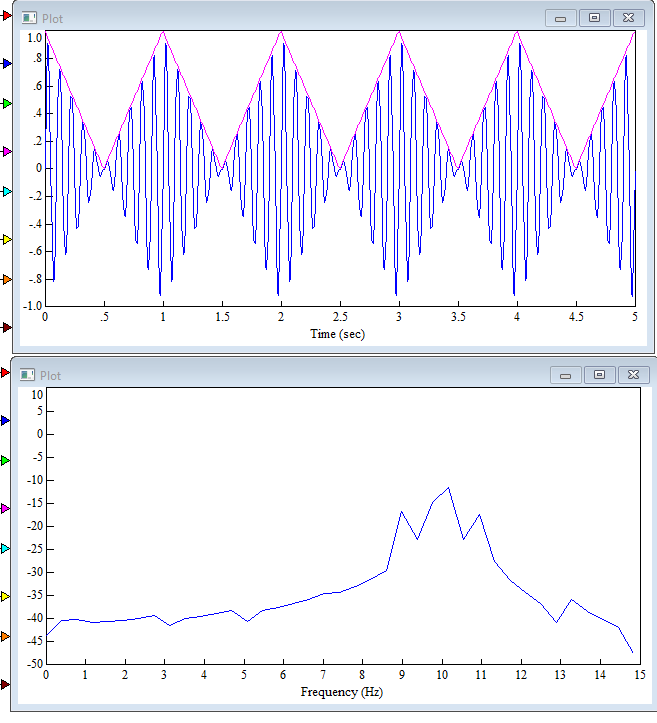
\includegraphics[width=0.6\textwidth]{Imagenes/Parte-3-moduladora-triangular-indice-de-modulacion-1.png}
    \caption{Señal AM con moduladora triangular e índice de modulación 1}
    \label{fig:parte3-triangular-indice-1}
\end{figure}

\begin{figure}[H]
    \centering
    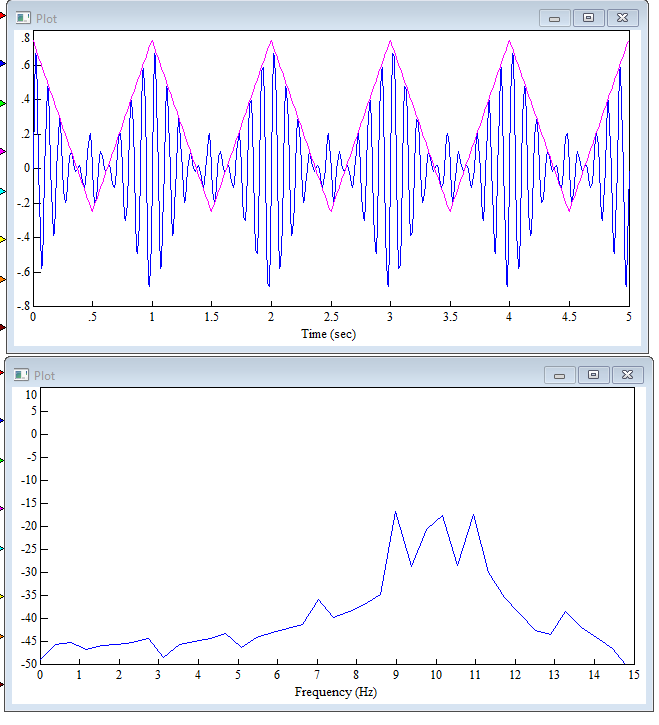
\includegraphics[width=0.6\textwidth]{Imagenes/Parte-3-moduladora-triangular-sobremodulacion.png}
    \caption{Señal AM con moduladora triangular en sobremodulación}
    \label{fig:parte3-triangular-sobremodulacion}
\end{figure}

%---------------------------------------------------------------
\subsection{Demodulación de una portadora, por el método coherente}

\begin{figure}[H]
    \centering
    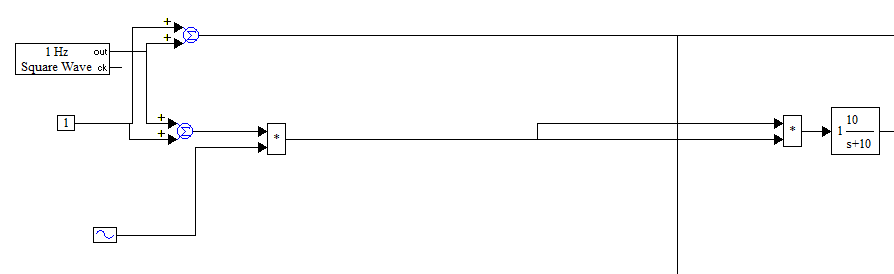
\includegraphics[width=0.6\textwidth]{Imagenes/parte-4-sistema-reconstructor-de-señal-modulada.png}
    \caption{Sistema reconstructor de la señal modulada mediante demodulación coherente}
    \label{fig:parte4-sistema-reconstructor}
\end{figure}

\begin{figure}[H]
    \centering
    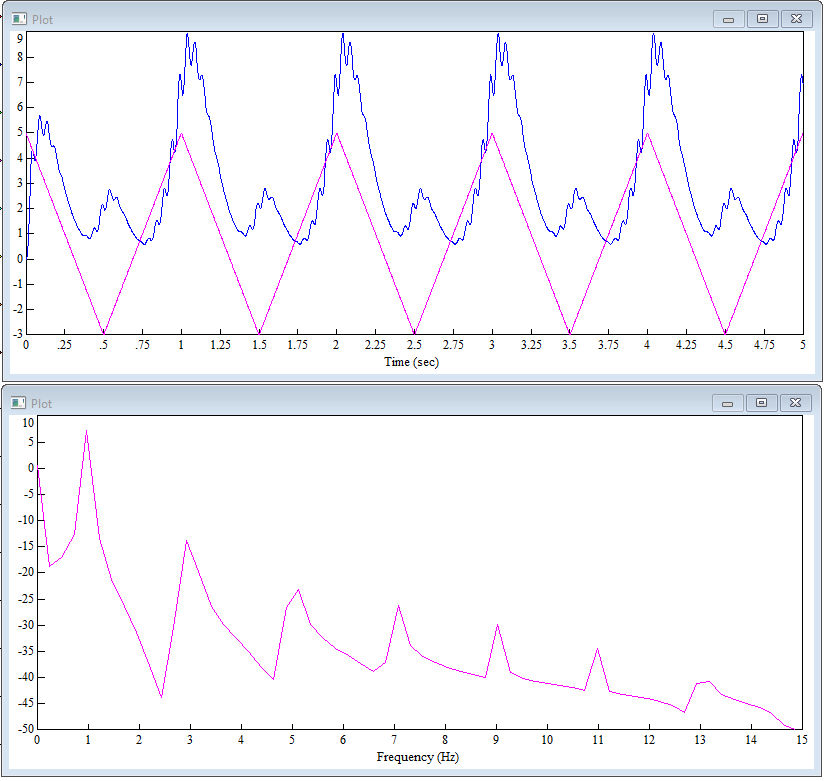
\includegraphics[width=0.6\textwidth]{Imagenes/parte-4-onda-triangular-reconstruida-sobremodulacion.png}
    \caption{Onda triangular demodulada y reconstruida en condición de sobremodulación}
    \label{fig:parte4-triangular-reconstruida-sobremodulacion}
\end{figure}

% Señal cuadrada reconstruida para distintas constantes de tiempo
\begin{figure}[H]
    \centering
    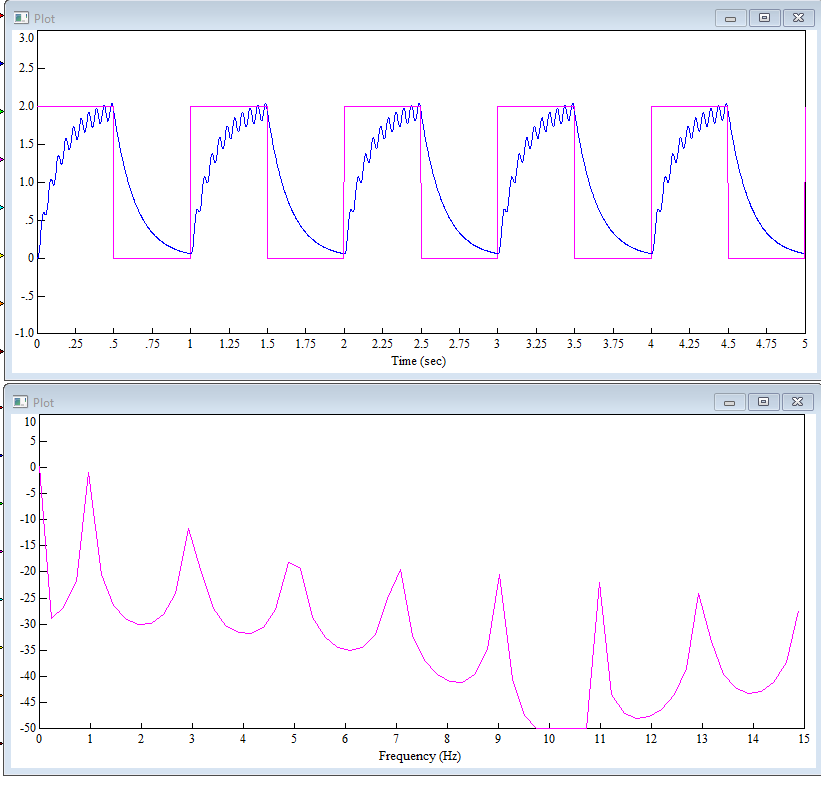
\includegraphics[width=0.6\textwidth]{Imagenes/parte-4-señal-cuadrada-reconstruida-constante-de-tiempo-7.png}
    \caption{Señal cuadrada demodulada y reconstruida con constante de tiempo 7}
    \label{fig:parte4-cuadrada-constante-7}
\end{figure}

\begin{figure}[H]
    \centering
    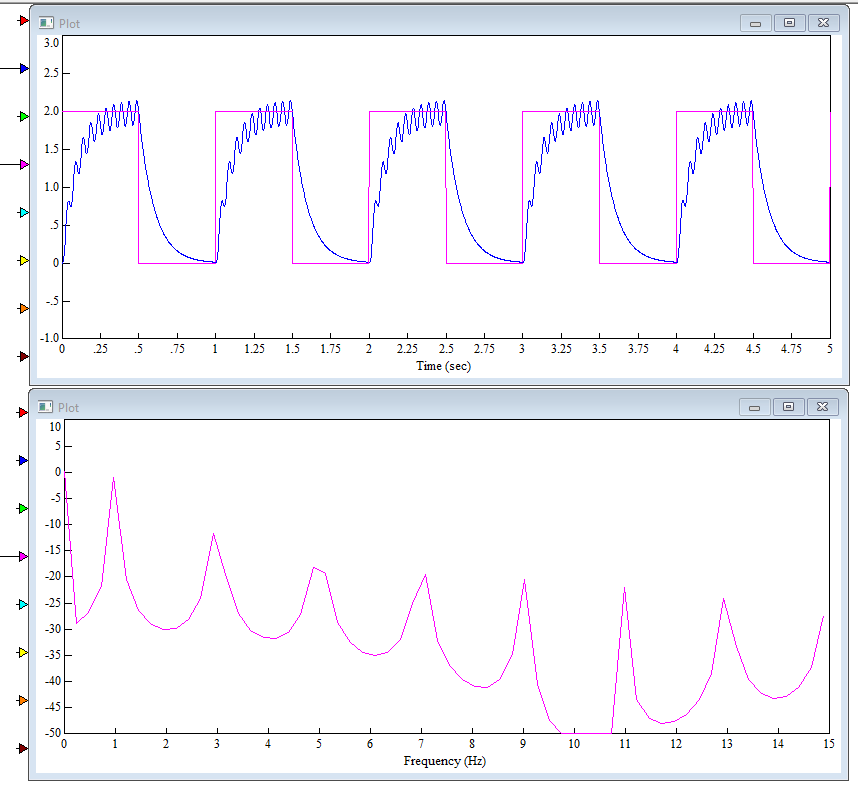
\includegraphics[width=0.6\textwidth]{Imagenes/parte-4-señal-cuadrada-reconstruida-constante-de-tiempo-10.png}
    \caption{Señal cuadrada demodulada y reconstruida con constante de tiempo 10}
    \label{fig:parte4-cuadrada-constante-10}
\end{figure}

\begin{figure}[H]
    \centering
    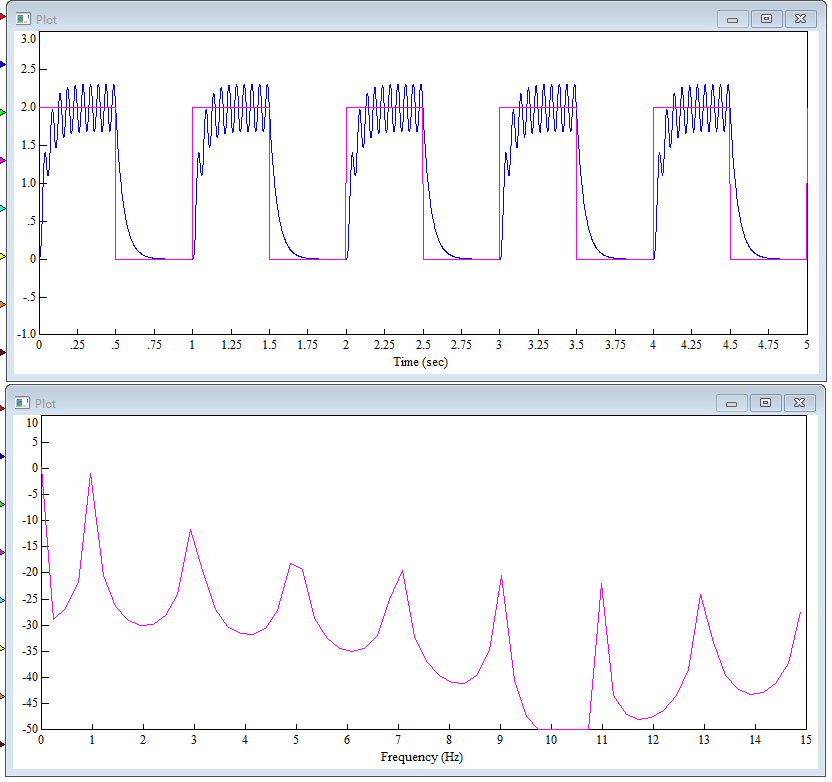
\includegraphics[width=0.6\textwidth]{Imagenes/parte-4-señal-cuadrada-reconstruida-constante-de-tiempo-20.png}
    \caption{Señal cuadrada demodulada y reconstruida con constante de tiempo 20}
    \label{fig:parte4-cuadrada-constante-20}
\end{figure}

% Señal diente de sierra reconstruida para distintas constantes de tiempo
\begin{figure}[H]
    \centering
    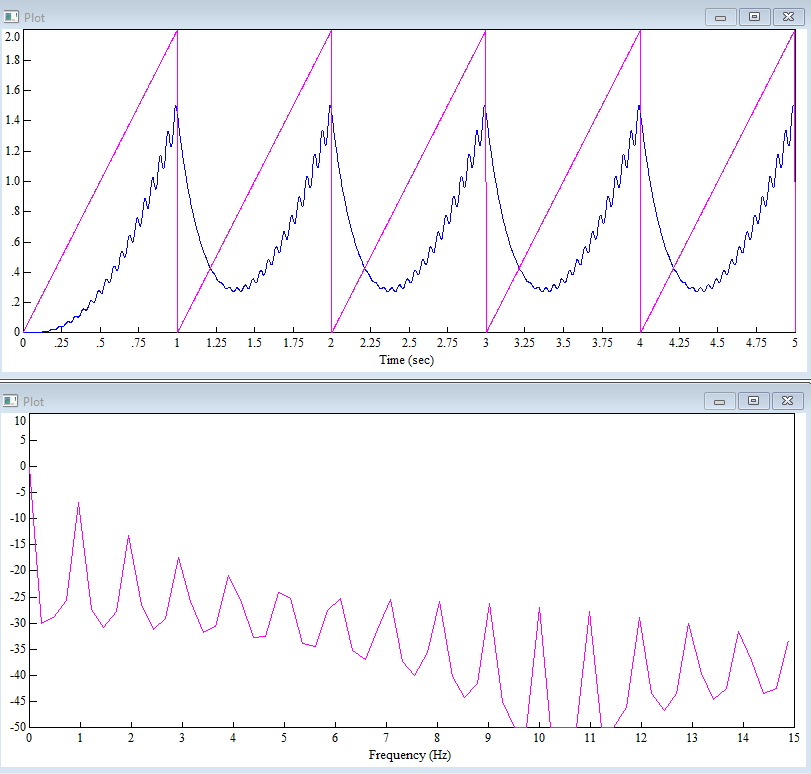
\includegraphics[width=0.6\textwidth]{Imagenes/parte-4-señal-dientedesierra-reconstruida-constante-de-tiempo-6.png}
    \caption{Señal diente de sierra demodulada y reconstruida con constante de tiempo 6}
    \label{fig:parte4-dientedesierra-constante-6}
\end{figure}

\begin{figure}[H]
    \centering
    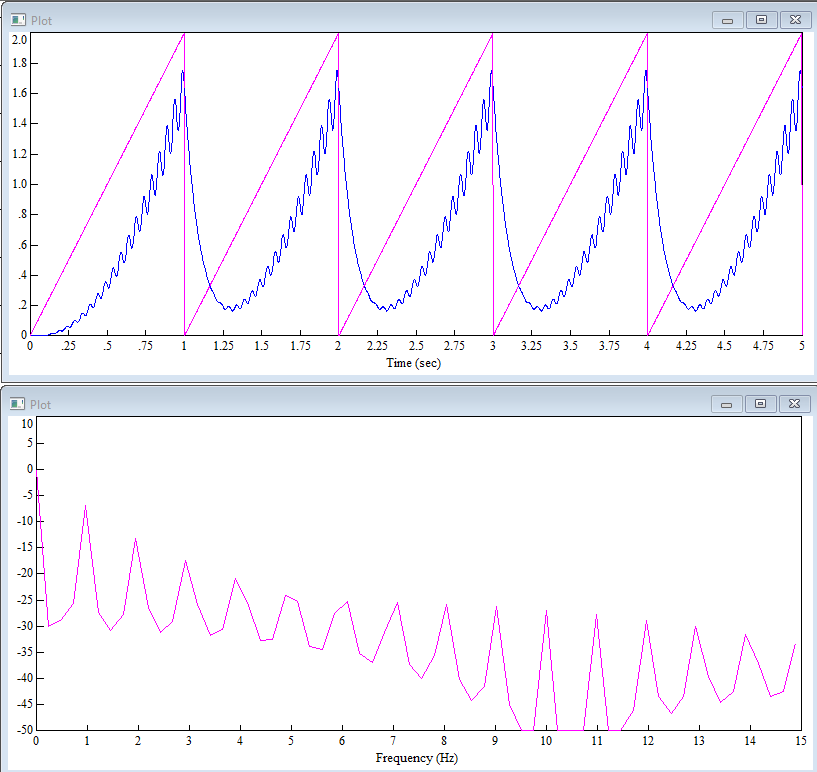
\includegraphics[width=0.6\textwidth]{Imagenes/parte-4-señal-dientedesierra-reconstruida-constante-de-tiempo-10.png}
    \caption{Señal diente de sierra demodulada y reconstruida con constante de tiempo 10}
    \label{fig:parte4-dientedesierra-constante-10}
\end{figure}

\begin{figure}[H]
    \centering
    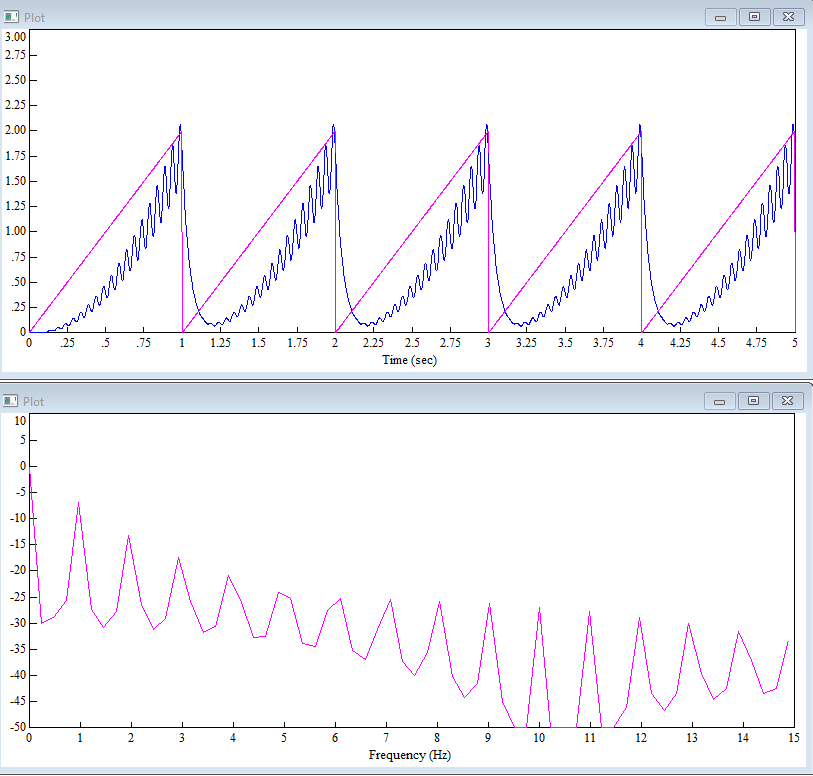
\includegraphics[width=0.6\textwidth]{Imagenes/parte-4-señal-dientedesierra-reconstruida-constante-de-tiempo-20.png}
    \caption{Señal diente de sierra demodulada y reconstruida con constante de tiempo 20}
    \label{fig:parte4-dientedesierra-constante-20}
\end{figure}

% Señal triangular reconstruida para distintas constantes de tiempo
\begin{figure}[H]
    \centering
    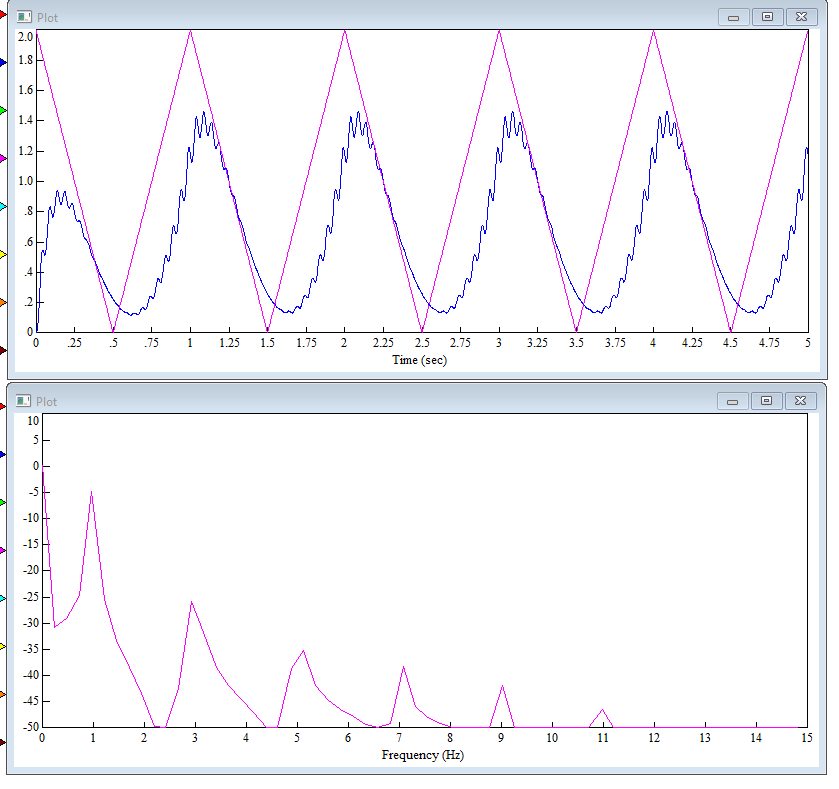
\includegraphics[width=0.6\textwidth]{Imagenes/parte-4-señal-triangular-reconstruida-constante-de-tiempo-7.png}
    \caption{Señal triangular demodulada y reconstruida con constante de tiempo 7}
    \label{fig:parte4-triangular-constante-7}
\end{figure}

\begin{figure}[H]
    \centering
    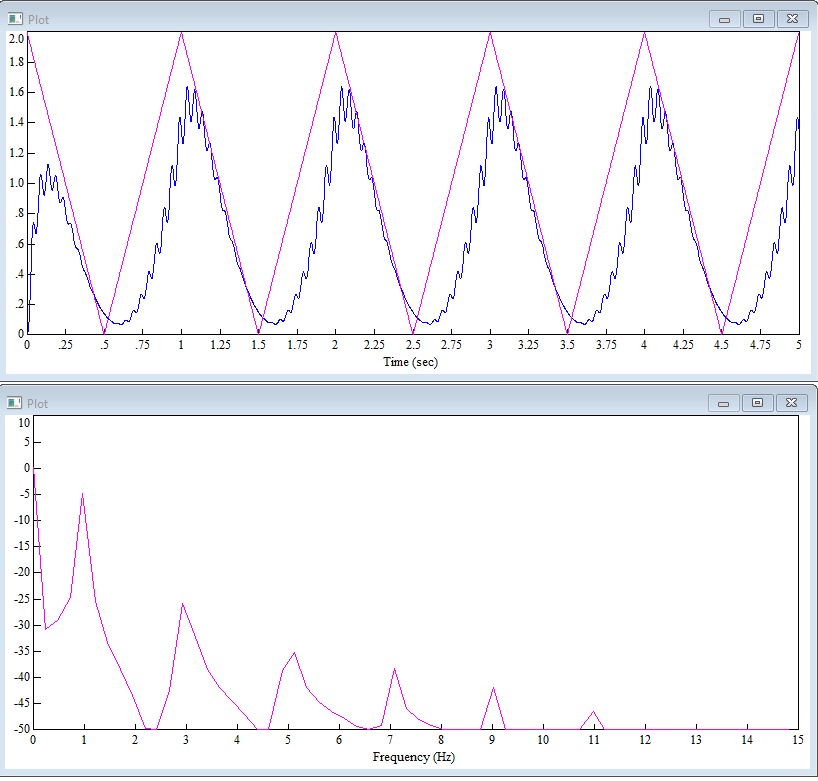
\includegraphics[width=0.6\textwidth]{Imagenes/parte-4-señal-triangular-reconstruida-constante-de-tiempo-10.png}
    \caption{Señal triangular demodulada y reconstruida con constante de tiempo 10}
    \label{fig:parte4-triangular-constante-10}
\end{figure}

\begin{figure}[H]
    \centering
    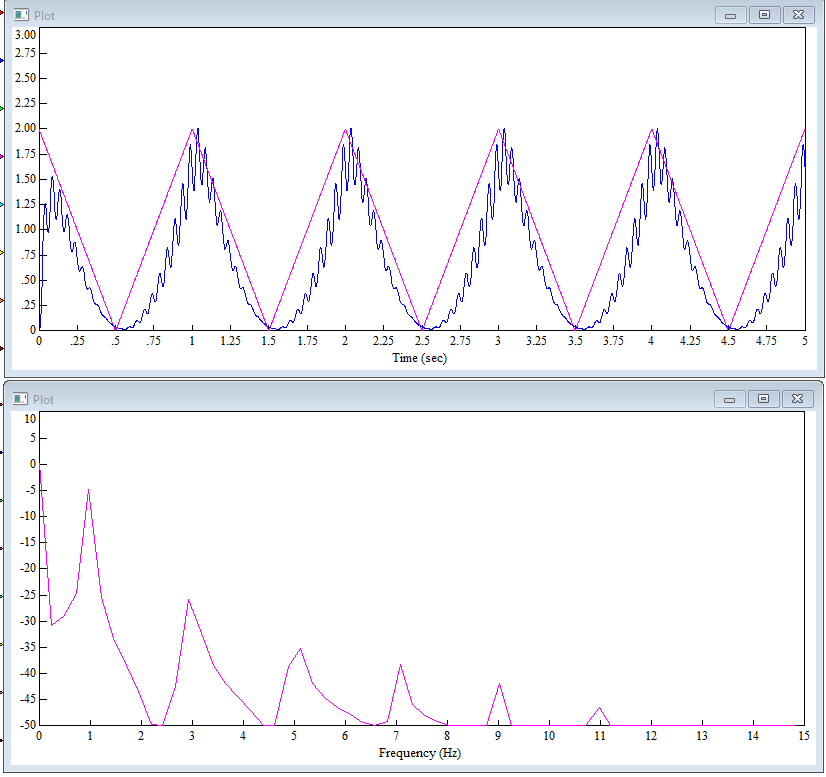
\includegraphics[width=0.6\textwidth]{Imagenes/parte-4-señal-triangular-reconstruida-constante-de-tiempo-20.png}
    \caption{Señal triangular demodulada y reconstruida con constante de tiempo 20}
    \label{fig:parte4-triangular-constante-20}
\end{figure}
